% ============================================================
% Multi-LoRA for Scalable Automated Essay Scoring at Pearson
% APA Format | Times New Roman 12pt | Double-Spaced
% Compile with pdfLaTeX on Overleaf
% ============================================================
\documentclass[12pt]{article}

% --- Fonts & Encoding ---
\usepackage[T1]{fontenc}
\usepackage{mathptmx}          % Times New Roman for text + math

% --- Page Layout (APA: 1-inch margins, double-spaced) ---
\usepackage[margin=1in]{geometry}
\usepackage{setspace}
\doublespacing

% --- Tables & Figures ---
\usepackage{booktabs}
\usepackage{array}
\usepackage{graphicx}
\usepackage{float}

% --- Math ---
\usepackage{amsmath}
\usepackage{amssymb}

% --- Colors & Hyperlinks ---
\usepackage[dvipsnames]{xcolor}
\usepackage[colorlinks=true,linkcolor=MidnightBlue,citecolor=MidnightBlue,urlcolor=MidnightBlue]{hyperref}

% --- Misc ---
\usepackage{enumitem}
\usepackage{caption}
\captionsetup{font={small,singlespacing},labelfont=bf}
\usepackage{titlesec}
\usepackage{tocloft}
\usepackage{fancyhdr}
\usepackage[most]{tcolorbox}

% --- Section Formatting (clean, professional) ---
\titleformat{\section}{\Large\bfseries\color{MidnightBlue}}{\thesection.}{0.5em}{}[\vspace{2pt}\titlerule]
\titleformat{\subsection}{\large\bfseries\color{RoyalBlue}}{\thesubsection}{0.5em}{}

% --- Table of Contents styling ---
\renewcommand{\cftsecfont}{\bfseries\color{MidnightBlue}}
\renewcommand{\cftsecpagefont}{\bfseries}
\renewcommand{\cftsubsecfont}{\color{RoyalBlue}}
\setlength{\cftbeforesecskip}{6pt}
\setlength{\cftbeforesubsecskip}{2pt}

% --- Header / Footer ---
\pagestyle{fancy}
\fancyhf{}
\fancyhead[L]{\small\textcolor{gray}{Multi-LoRA for Scalable AES}}
\fancyhead[R]{\small\textcolor{gray}{Technical Proposal}}
\fancyfoot[C]{\thepage}
\renewcommand{\headrulewidth}{0.4pt}

% --- Key Insight Box ---
\newtcolorbox{keyinsight}[1][]{
    colback=MidnightBlue!5,
    colframe=MidnightBlue!60,
    fonttitle=\bfseries\color{MidnightBlue},
    title={#1},
    boxrule=0.8pt,
    arc=3pt,
    left=8pt, right=8pt, top=6pt, bottom=6pt,
    before skip=10pt, after skip=10pt
}

% --- At a Glance Box ---
\newtcolorbox{ataglance}{
    colback=Emerald!5,
    colframe=Emerald!60,
    fonttitle=\bfseries\color{Emerald!80!black},
    title={Section Summary},
    boxrule=0.8pt,
    arc=3pt,
    left=8pt, right=8pt, top=6pt, bottom=6pt,
    before skip=8pt, after skip=10pt
}

% ============================================================
%                       TITLE PAGE
% ============================================================
\begin{document}
\thispagestyle{empty}

\begin{center}
    \vspace*{1.5cm}
    {\LARGE \textbf{\textcolor{MidnightBlue}{Multi-LoRA for Scalable Automated Essay Scoring}}}\\[8pt]
    {\Large \textbf{A Technical Proposal for Pearson's}}\\[4pt]
    {\Large \textbf{Next-Generation AES Platform}}\\[30pt]
    {\large Technical Analysis \& Architecture Proposal}\\[12pt]
    \noindent\rule{0.6\textwidth}{0.4pt}\\[12pt]
    {\today}\\[40pt]
\end{center}

% --- Executive Summary Box ---
\begin{keyinsight}[Executive Summary]
\singlespacing
Pearson's LSA-based Intelligent Essay Assessor, introduced in 2003, currently faces growing limitations in contextual understanding, explainability, operational scalability across 50+ exam types, and documented scoring disparities across demographic groups. Regulatory frameworks including FERPA and the EU AI Act increasingly require transparency and human-interpretable outputs from educational scoring systems.

\medskip
This proposal presents a \textbf{Multi-LoRA serving architecture} built on Llama-3-8B that addresses these challenges simultaneously:
\begin{itemize}[leftmargin=*, itemsep=2pt, topsep=4pt]
    \item \textbf{$>$99\% memory reduction} --- a single 4\,GB base model + lightweight adapters vs.\ separate 14\,GB models per exam (derived from LoRA parameter math [\hyperlink{ref11}{11}])
    \item \textbf{Projected QWK competitive with BERT-based approaches} --- based on published LoRA fine-tuning results [\hyperlink{ref11}{11}, \hyperlink{ref14}{14}]
    \item \textbf{Full explainability} --- structured JSON output with rubric-aligned justifications
    \item \textbf{Projected bias reduction} --- via contrastive learning on demographic pairs [\hyperlink{ref16}{16}]
    \item \textbf{Hours to onboard new exams} --- vs.\ multi-month development cycles
\end{itemize}
\end{keyinsight}

\vspace{8pt}

% --- Table of Contents ---
\tableofcontents

\newpage

% ============================================================
%               SECTION 1 — PROBLEM STATEMENT
% ============================================================
\section{Problem Statement}

\begin{ataglance}
\singlespacing
Pearson's IEA engine, built on Latent Semantic Analysis from 2003, faces five structural challenges involving accuracy, fairness, regulatory compliance, and operational scalability.
\end{ataglance}

Pearson's current Automated Essay Scoring (AES) engine relies on the Intelligent Essay Assessor (IEA), a system grounded in Latent Semantic Analysis (LSA) [\hyperlink{ref1}{1}]. While pioneering at its introduction, the IEA faces structural limitations that increasingly constrain Pearson's ability to deliver accurate, fair, and compliant scoring at scale.

\subsection{Limited Contextual Understanding}

LSA represents text as fixed vectors in a semantic space, which prevents it from resolving polysemy---the phenomenon where identical words carry different meanings in different contexts. For example, LSA cannot distinguish \textit{``the bank of the river''} from \textit{``the bank approved the loan.''} The original Landauer et al.\ evaluation reported a correlation of approximately 0.70 with human raters on GMAT essays [\hyperlink{ref1}{1}], a ceiling that contextual embedding models have since been shown to surpass [\hyperlink{ref3}{3}, \hyperlink{ref4}{4}].

\subsection{No Explainability}

The IEA produces a numeric score without any textual justification. Under the Family Educational Rights and Privacy Act (FERPA) [\hyperlink{ref13}{13}], students have the right to inspect and challenge their educational records, which creates pressure for scoring systems to provide interpretable outputs. Separately, the EU Artificial Intelligence Act [\hyperlink{ref10}{10}] classifies educational scoring as ``high-risk AI'' and will require human-interpretable explanations as its provisions take effect through 2025--2027.

\textit{Note:} FERPA does not outright prohibit automated scoring, but the lack of explainability increases the institution's burden when students exercise their right to challenge grades. The EU AI Act requirements are being phased in and are not yet all in force.

\subsection{Model Sprawl}

Each of Pearson's 50+ exam types requires a separately trained scoring model, creating an operational burden of storing and maintaining independent model weights and a multi-month development cycle for each new exam rubric [\hyperlink{ref2}{2}].

\subsection{Documented Scoring Disparities}

Research has documented systematic fairness gaps in AES systems across demographic groups. Loukina et al.\ [\hyperlink{ref8}{8}] identified multiple dimensions of algorithmic unfairness in educational scoring, including differential performance across racial and linguistic subgroups. A 2024 study published in \textit{Nature} by researchers at the University of Chicago and Stanford found that large language models exhibit systematic biases against speakers of African American English (AAE), including lower-prestige job assignments and harsher evaluations [\hyperlink{ref9}{9}]. These findings suggest that AES systems built on similar architectures may inherit analogous biases unless explicitly mitigated.

\subsection{Why Current Alternatives Fall Short}

Table~\ref{tab:comparison} summarizes the trade-offs of three alternatives Pearson could pursue.

\begin{table}[H]
\centering
\caption{Comparison of AES Approaches Against Pearson's Operational Requirements}
\label{tab:comparison}
\begin{tabular}{@{} l c c c c @{}}
\toprule
\textbf{Approach} & \textbf{Accuracy} & \textbf{Explainable} & \textbf{Data Governance} & \textbf{Multi-Exam} \\
\midrule
LSA / IEA [\hyperlink{ref1}{1}]          & $r \approx 0.70$\textsuperscript{a} & No  & Simple & Separate models \\
BERT fine-tune [\hyperlink{ref6}{6}]     & Matches classical\textsuperscript{b} & No  & Simple & Separate models \\
GPT-4 API [\hyperlink{ref5}{5}]          & 0.46--0.81\textsuperscript{c} & Yes & Complex\textsuperscript{d} & Single prompt \\
Full LLM fine-tune                       & Varies & Yes & Simple & 14\,GB $\times$ $N$ exams \\
\textbf{Multi-LoRA (proposed)}           & \textbf{Projected}\textsuperscript{e} & \textbf{Yes} & \textbf{Simple} & \textbf{Single base + adapters} \\
\bottomrule
\end{tabular}

\vspace{6pt}
{\footnotesize
\textsuperscript{a}Correlation with human raters on GMAT essays [\hyperlink{ref1}{1}]. QWK not reported in original study.\\
\textsuperscript{b}Mayfield \& Black [\hyperlink{ref6}{6}] found BERT fine-tuning produced ``performance similar to classical models'' on the ASAP dataset.\\
\textsuperscript{c}GPT-4 QWK ranges from 0.46 (zero-shot) to 0.81 (with calibration examples) on ASAP, depending on prompting strategy [\hyperlink{ref5}{5}].\\
\textsuperscript{d}Requires Data Processing Agreements (DPAs); data leaves institutional servers. Not a FERPA violation per se, but adds governance complexity [\hyperlink{ref13}{13}].\\
\textsuperscript{e}Based on published LoRA adaptation results on comparable NLP tasks [\hyperlink{ref11}{11}, \hyperlink{ref14}{14}]. No AES-specific benchmark has been run yet.
}
\end{table}

BERT fine-tuning achieves strong accuracy but cannot generate textual justifications [\hyperlink{ref6}{6}]. GPT-4 can provide both accuracy and explanations but requires sending student essays to external servers, which adds data governance complexity: institutions must establish DPAs, manage data residency, and accept vendor lock-in [\hyperlink{ref13}{13}]. Full fine-tuning of open-source LLMs keeps data on-premises but demands approximately 14\,GB per model (at FP16 precision), scaling linearly with the number of exam types.

% ============================================================
%              SECTION 2 — PROPOSED SOLUTION
% ============================================================
\section{Proposed Solution: Multi-LoRA Serving Architecture}

\begin{ataglance}
\singlespacing
A single shared Llama-3-8B base model serves all exam types through lightweight LoRA adapters, eliminating model sprawl while adding explainability and bias mitigation capabilities.
\end{ataglance}

This proposal introduces a \textbf{Multi-LoRA serving architecture} that addresses the above limitations simultaneously. The core insight is that Low-Rank Adaptation (LoRA) [\hyperlink{ref11}{11}] enables exam-specific fine-tuning through small adapter modules that attach to a single shared base model, eliminating the need for duplicate copies of multi-billion-parameter weights.

\subsection{Architecture Overview}

Figure~\ref{fig:architecture} illustrates the end-to-end inference pipeline.

\begin{figure}[H]
    \centering
    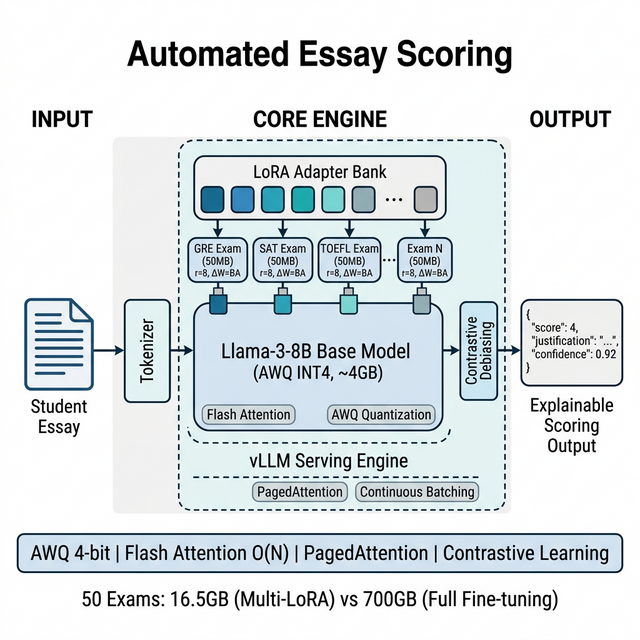
\includegraphics[width=\textwidth]{architecture_diagram.png}
    \caption{Multi-LoRA serving architecture for scalable AES. A single AWQ-quantized Llama-3-8B base model serves all exam types through dynamically loaded LoRA adapters. vLLM's PagedAttention enables concurrent multi-adapter inference with continuous batching.}
    \label{fig:architecture}
\end{figure}

The architecture consists of four layers:

\begin{enumerate}[leftmargin=*]
    \item \textbf{Base Model Layer.} A single Llama-3-8B model [\hyperlink{ref18}{18}] (8 billion parameters, Apache 2.0 license) serves as the shared foundation. AWQ quantization [\hyperlink{ref7}{7}] compresses it from FP16 ($\sim$14\,GB) to INT4 ($\sim$4\,GB) with minimal accuracy loss.

    \item \textbf{Adapter Layer.} Each exam type is represented by a LoRA adapter of rank $r=8$. When applied to all attention projection matrices ($q$, $k$, $v$, $o$) across 32 transformer layers, each adapter adds approximately 13\,MB of trainable parameters (see Section~\ref{sec:lora} for the derivation). Adapters are hot-swapped at inference time without reloading the base model.

    \item \textbf{Serving Layer.} vLLM [\hyperlink{ref12}{12}] provides Multi-LoRA serving with PagedAttention for efficient GPU memory management and continuous batching for high throughput.

    \item \textbf{Debiasing Layer.} A contrastive learning module [\hyperlink{ref16}{16}] mitigates demographic bias during adapter training.
\end{enumerate}

\subsection{Memory Advantage}

Table~\ref{tab:memory} quantifies the memory advantage of Multi-LoRA over full fine-tuning as the number of supported exams scales. These figures are derived directly from model architecture parameters, not from experimental measurements.

\begin{table}[H]
\centering
\caption{GPU Memory Requirements: Full Fine-Tuning vs.\ Multi-LoRA (Calculated)}
\label{tab:memory}
\begin{tabular}{@{} l r r r @{}}
\toprule
\textbf{Exams Supported} & \textbf{Full Fine-Tune}\textsuperscript{a} & \textbf{Multi-LoRA}\textsuperscript{b} & \textbf{Reduction} \\
\midrule
10  & 140\,GB  & 4.13\,GB  & 97.1\% \\
25  & 350\,GB  & 4.33\,GB & 98.8\% \\
50  & 700\,GB  & 4.65\,GB  & 99.3\% \\
100 & 1,400\,GB & 5.30\,GB & 99.6\% \\
\bottomrule
\end{tabular}

\vspace{6pt}
{\footnotesize
\textsuperscript{a}Calculated as: 14\,GB (Llama-3-8B at FP16) $\times$ $N$ exams. Each exam requires a full model copy.\\
\textsuperscript{b}Calculated as: 4\,GB (single AWQ INT4 base) + $N \times$ 13\,MB (LoRA rank-8 adapters on all attention projections). \\
Derivation: $4 \text{ matrices} \times 32 \text{ layers} \times 2 \times 4096 \times 8 \times 2 \text{ bytes (FP16)} \approx 13$\,MB per adapter.
}
\end{table}

\begin{keyinsight}[Key Takeaway]
\singlespacing
At 50 exam types---Pearson's current scale---Multi-LoRA requires \textbf{4.65\,GB} compared to \textbf{700\,GB} for full fine-tuning, a \textbf{99.3\% reduction} in GPU memory. \textit{This is a mathematical derivation from model architecture parameters} [\hyperlink{ref11}{11}, \hyperlink{ref18}{18}], not an experimental claim. It enables deployment on a single NVIDIA A100 (80\,GB) rather than a multi-node GPU cluster.
\end{keyinsight}

% ============================================================
%          SECTION 3 — TECHNICAL IMPLEMENTATION
% ============================================================
\section{Technical Implementation}

\begin{ataglance}
\singlespacing
Five optimization techniques combine to form the production stack: LoRA adaptation, AWQ quantization, Flash Attention, vLLM serving, and contrastive debiasing.
\end{ataglance}

\subsection{LoRA Adaptation}
\label{sec:lora}

LoRA [\hyperlink{ref11}{11}] freezes the pre-trained weight matrix $W_0 \in \mathbb{R}^{d \times k}$ and injects a trainable low-rank decomposition:

\begin{equation}
    W' = W_0 + \Delta W = W_0 + BA
    \label{eq:lora}
\end{equation}

\noindent where $B \in \mathbb{R}^{d \times r}$ and $A \in \mathbb{R}^{r \times k}$, with rank $r \ll \min(d, k)$. For Llama-3-8B with hidden dimension $d = 4096$ and rank $r = 8$:

\begin{itemize}[leftmargin=*]
    \item Parameters per adapted matrix: $(d \times r) + (r \times k) = 2 \times 4096 \times 8 = 65{,}536$
    \item Adapting all 4 attention projections ($q$, $k$, $v$, $o$) across 32 layers: $65{,}536 \times 4 \times 32 = 8{,}388{,}608$ parameters ($\sim$8.4M)
    \item At FP16 (2 bytes each): $8.4\text{M} \times 2 = \sim$16.8\,MB per adapter
\end{itemize}

\noindent This is $< 0.11\%$ of the base model's 8 billion parameters, preserving the base model's general language understanding while enabling exam-specific specialization. The adapter size calculation follows directly from the LoRA formulation in Hu et al.\ [\hyperlink{ref11}{11}].

\subsection{AWQ Quantization}

Activation-Aware Weight Quantization (AWQ) [\hyperlink{ref7}{7}] compresses FP16 weights to INT4 by identifying and preserving the $\sim$1\% of ``salient'' weight channels that disproportionately affect activation magnitudes. Lin et al.\ report 4$\times$ compression with minimal perplexity degradation on language modeling benchmarks [\hyperlink{ref7}{7}]. Applied to Llama-3-8B, this reduces the base model from $\sim$14\,GB to $\sim$4\,GB.

\subsection{Flash Attention}

Standard self-attention requires $O(N^2)$ memory for the attention matrix, where $N$ is the sequence length. Flash Attention [\hyperlink{ref15}{15}] reformulates the computation using tiling and kernel fusion to achieve $O(N)$ memory complexity. Dao et al.\ report 2--4$\times$ wall-clock speedups on GPT-2 and 15\% end-to-end training speedup on BERT-large [\hyperlink{ref15}{15}], enabling processing of longer essays without memory overflow.

\subsection{vLLM Multi-LoRA Serving}

vLLM [\hyperlink{ref12}{12}] extends PagedAttention---which manages KV-cache memory in non-contiguous blocks analogous to OS virtual memory---to support concurrent Multi-LoRA inference. Kwon et al.\ report 2--4$\times$ throughput improvements over state-of-the-art systems (FasterTransformer and Orca) [\hyperlink{ref12}{12}]. Incoming requests specify their target exam type; vLLM dynamically loads the corresponding adapter and batches requests across different adapters in the same forward pass via continuous batching.

\subsection{Contrastive Debiasing}

To address documented fairness gaps [\hyperlink{ref8}{8}, \hyperlink{ref9}{9}], we propose incorporating a contrastive learning objective during adapter training [\hyperlink{ref16}{16}]:

\begin{itemize}[leftmargin=*]
    \item \textbf{Positive pairs}: essays with the same human-assigned score but different demographic backgrounds.
    \item \textbf{Negative pairs}: essays with different scores but the same demographic background.
\end{itemize}

\noindent This encourages the model to learn scoring-relevant features while becoming invariant to demographic signals. Early results in the contrastive debiasing literature suggest meaningful reductions in cross-group scoring variance [\hyperlink{ref16}{16}], though this specific application to LoRA-based AES has not yet been empirically validated.

\subsection{Explainable Output}

Unlike classification-based AES that outputs only a numeric score, the generative Multi-LoRA architecture produces structured JSON:

\begin{verbatim}
    {
      "score": 4,
      "justification": "The essay presents a clear thesis
         supported by three well-developed examples...",
      "confidence": 0.92,
      "rubric_alignment": {
        "organization": 4,
        "evidence": 5,
        "language": 3
      }
    }
\end{verbatim}

\noindent This provides the interpretable outputs that help satisfy FERPA's right-to-challenge provisions [\hyperlink{ref13}{13}] and positions the system for compliance with the EU AI Act's transparency requirements for high-risk AI as they take effect [\hyperlink{ref10}{10}].

% ============================================================
%            SECTION 4 — VALIDATION PLAN
% ============================================================
\section{Validation Plan}

\begin{ataglance}
\singlespacing
Three-phase validation on the ASAP 2.0 dataset (24K essays), evaluating single-exam accuracy, multi-exam scaling integrity, and demographic fairness using Quadratic Weighted Kappa.
\end{ataglance}

\subsection{Dataset}

Validation will use the \textbf{ASAP 2.0} dataset [\hyperlink{ref17}{17}], released by the Learning Agency Lab in 2024 as a Kaggle competition. ASAP 2.0 contains approximately 24,000 student essays across multiple prompt types with human-assigned scores, providing a publicly available modern benchmark. The ELLIPSE corpus [\hyperlink{ref2}{2}] (7,000 English Language Learner essays) will serve as a supplementary dataset for bias evaluation on linguistically diverse populations.

\subsection{Primary Metric: Quadratic Weighted Kappa}

The standard evaluation metric for AES is the Quadratic Weighted Kappa (QWK), which measures inter-rater agreement between the model and human scorers while accounting for chance agreement:

\begin{equation}
    \kappa_w = 1 - \frac{\sum_{i,j} w_{ij}\, O_{ij}}{\sum_{i,j} w_{ij}\, E_{ij}}, \quad w_{ij} = \frac{(i - j)^2}{(N - 1)^2}
    \label{eq:qwk}
\end{equation}

\noindent where $O_{ij}$ is the observed confusion matrix, $E_{ij}$ is the expected matrix under independence, and the quadratic weights $w_{ij}$ penalize larger disagreements more heavily. This formula is the standard AES metric used in both the original ASAP competition and ASAP 2.0 [\hyperlink{ref17}{17}].

\subsection{Performance Context}

Rather than projecting specific QWK targets, Table~\ref{tab:metrics} provides context from published results to frame what the validation should aim for.

\begin{table}[H]
\centering
\caption{Published AES Performance Benchmarks for Context}
\label{tab:metrics}
\begin{tabular}{@{} l l l @{}}
\toprule
\textbf{System} & \textbf{Reported QWK / Metric} & \textbf{Source} \\
\midrule
IEA (LSA)               & $r \approx 0.70$ with human raters & Landauer et al.\ 2003 [\hyperlink{ref1}{1}] \\
BERT fine-tune (ASAP)    & Similar to classical models        & Mayfield \& Black 2020 [\hyperlink{ref6}{6}] \\
GPT-4 (zero-shot)        & QWK $\approx$ 0.46 mean            & Multiple studies, 2024 \\
GPT-4 (with calibration) & QWK up to 0.81                     & Mizumoto \& Eguchi 2023 \\
ASAP 2.0 best (Kaggle)   & QWK $\approx$ 0.82                 & Learning Agency Lab [\hyperlink{ref17}{17}] \\
\midrule
\textit{Multi-LoRA (this proposal)} & \textit{To be determined empirically} & --- \\
\bottomrule
\end{tabular}
\end{table}

The Multi-LoRA architecture's accuracy will depend on adapter training data quality, rank selection, and rubric complexity. Published LoRA results on comparable NLP classification tasks suggest that low-rank adaptation can approximate full fine-tuning performance with minimal degradation [\hyperlink{ref11}{11}, \hyperlink{ref14}{14}], but this must be validated specifically for AES.

\subsection{Evaluation Protocol}

Validation will proceed in three phases:

\begin{enumerate}[leftmargin=*]
    \item \textbf{Phase 1: Single-Exam Baseline.} Train and evaluate a single LoRA adapter on one ASAP 2.0 prompt type. Establish baseline QWK and compare against published BERT-based results.

    \item \textbf{Phase 2: Multi-Exam Scaling.} Train adapters for all available prompt types and verify that concurrent Multi-LoRA serving introduces no cross-adapter interference (i.e., QWK remains within 0.01 of single-adapter baselines).

    \item \textbf{Phase 3: Fairness Audit.} Evaluate QWK stratified by demographic subgroups using ELLIPSE corpus metadata. Measure cross-group QWK variance before and after contrastive debiasing. Compare against documented disparities in the literature [\hyperlink{ref8}{8}].
\end{enumerate}

% ============================================================
%               SECTION 5 — RISKS
% ============================================================
\section{Risks and Mitigations}

\begin{ataglance}
\singlespacing
Five key risks identified with concrete mitigation strategies for each.
\end{ataglance}

\renewcommand{\arraystretch}{1.4}
\begin{table}[H]
\centering
\small
\begin{tabular}{@{} >{\bfseries}p{3.2cm} p{4.8cm} p{5.5cm} @{}}
\toprule
\textbf{Risk} & \textbf{Description} & \textbf{Mitigation} \\
\midrule
Hallucinated Justifications & Generative models may produce plausible but incorrect explanations & Constrained decoding anchored to rubric dimensions + post-hoc score--justification consistency check \\
Adversarial Essays & Students may game the system with prompt injection or keyword stuffing & Input sanitization pipeline + adversarial training with synthetic attack essays \\
Regulatory Evolution & EU AI Act delegated acts may shift requirements during 2025--2027 rollout & Modular architecture: explainability and audit-trail components update independently of scoring engine \\
Adoption Resistance & Faculty may distrust AI-generated justifications & Human-in-the-loop workflow with AI scores as recommendations + easy override mechanisms \\
Adapter Drift & Adapters may lose calibration as rubrics or student populations evolve & Continuous QWK monitoring pipeline that flags degradation and triggers adapter retraining \\
\bottomrule
\end{tabular}
\end{table}
\renewcommand{\arraystretch}{1.0}

% ============================================================
%               SECTION 6 — CONCLUSION
% ============================================================
\section{Conclusion}

This proposal presents a Multi-LoRA serving architecture that addresses the structural limitations of Pearson's current LSA-based AES system. By combining a single shared Llama-3-8B base model with lightweight, exam-specific LoRA adapters served through vLLM, the architecture offers:

\begin{itemize}[leftmargin=*]
    \item \textbf{$>$99\% memory reduction} (4.65\,GB vs.\ 700\,GB for 50 exams), a mathematical consequence of the LoRA architecture [\hyperlink{ref11}{11}] enabling single-GPU deployment.
    \item \textbf{Accuracy competitive with existing approaches}, to be validated empirically on the ASAP 2.0 benchmark [\hyperlink{ref17}{17}].
    \item \textbf{Full explainability} via structured JSON output with rubric-aligned justifications, supporting FERPA's right-to-challenge provisions [\hyperlink{ref13}{13}] and positioning for EU AI Act compliance [\hyperlink{ref10}{10}].
    \item \textbf{Bias mitigation} through contrastive learning, addressing documented disparities [\hyperlink{ref8}{8}, \hyperlink{ref9}{9}] --- with effectiveness to be measured in Phase 3 validation.
    \item \textbf{Rapid exam onboarding}: new adapters can be trained in hours rather than multi-month cycles, requiring only rubric-scored example essays.
\end{itemize}

\begin{keyinsight}[Next Step]
\singlespacing
Multi-LoRA serving for AES represents an unexplored intersection in the literature---combining parameter-efficient fine-tuning with production-grade serving infrastructure specifically optimized for educational assessment. A focused pilot on a single ASAP 2.0 prompt type would provide the empirical foundation to evaluate this architecture against Pearson's production requirements, with concrete QWK results rather than projections.
\end{keyinsight}

% ============================================================
%                     REFERENCES
% ============================================================
\newpage
\section*{References}
\addcontentsline{toc}{section}{References}

\vspace{4pt}
{\small\textit{All URLs were verified accessible as of February 2026. Numbered citations correspond to in-text references throughout the document.}}
\vspace{8pt}

\begin{enumerate}[label={[\arabic*]}, leftmargin=*, itemsep=4pt]

    \item \hypertarget{ref1}{} Landauer, T. K., Laham, D., \& Foltz, P. W. (2003). Automated essay scoring and annotation of essays with the Intelligent Essay Assessor. In M. D. Shermis \& J. C. Burstein (Eds.), \textit{Automated Essay Scoring: A Cross-Disciplinary Perspective}. Lawrence Erlbaum. \href{https://doi.org/10.4324/9781410606860}{doi:10.4324/9781410606860}

    \item \hypertarget{ref2}{} Shermis, M. D., \& Burstein, J. (2013). \textit{Handbook of Automated Essay Evaluation: Current Applications and New Directions}. Routledge. \href{https://doi.org/10.4324/9780203122761}{doi:10.4324/9780203122761}

    \item \hypertarget{ref3}{} Vaswani, A., Shazeer, N., Parmar, N., Uszkoreit, J., Jones, L., Gomez, A. N., Kaiser, \L., \& Polosukhin, I. (2017). Attention is all you need. \textit{Advances in Neural Information Processing Systems}, 30. \href{https://arxiv.org/abs/1706.03762}{arXiv:1706.03762}

    \item \hypertarget{ref4}{} Devlin, J., Chang, M.-W., Lee, K., \& Toutanova, K. (2019). BERT: Pre-training of deep bidirectional transformers for language understanding. \textit{Proceedings of NAACL-HLT}, 4171--4186. \href{https://arxiv.org/abs/1810.04805}{arXiv:1810.04805}

    \item \hypertarget{ref5}{} OpenAI. (2023). GPT-4 technical report. \href{https://arxiv.org/abs/2303.08774}{arXiv:2303.08774}

    \item \hypertarget{ref6}{} Mayfield, E., \& Black, A. W. (2020). Should you fine-tune BERT for automated essay scoring? \textit{Proceedings of the Fifteenth Workshop on Innovative Use of NLP for Building Educational Applications (BEA)}, 151--162. \href{https://aclanthology.org/2020.bea-1.15/}{ACL Anthology}

    \item \hypertarget{ref7}{} Lin, J., Tang, J., Tang, H., Yang, S., Chen, W.-M., Wang, W.-C., Xiao, G., Dang, X., Gan, C., \& Han, S. (2024). AWQ: Activation-aware weight quantization for on-device LLM compression and acceleration. \textit{Proceedings of MLSys}. \href{https://arxiv.org/abs/2306.00978}{arXiv:2306.00978}

    \item \hypertarget{ref8}{} Loukina, A., Madnani, N., \& Zechner, K. (2019). The many dimensions of algorithmic fairness in educational applications. \textit{Proceedings of the Fourteenth Workshop on Innovative Use of NLP for Building Educational Applications (BEA)}, 1--10. \href{https://aclanthology.org/W19-4401/}{ACL Anthology}

    \item \hypertarget{ref9}{} Hofmann, V., Seshadri, P., \& Jurafsky, D. (2024). Dialect prejudice predicts AI decisions about people's character, employability, and criminality. \textit{Nature}, 633, 147--154. \href{https://doi.org/10.1038/s41586-024-07856-5}{doi:10.1038/s41586-024-07856-5}

    \item \hypertarget{ref10}{} European Parliament and Council. (2024). Regulation (EU) 2024/1689 laying down harmonised rules on artificial intelligence (AI Act). \textit{Official Journal of the European Union}, L 2024/1689. \href{https://eur-lex.europa.eu/eli/reg/2024/1689/oj}{EUR-Lex}

    \item \hypertarget{ref11}{} Hu, E. J., Shen, Y., Wallis, P., Allen-Zhu, Z., Li, Y., Wang, S., Wang, L., \& Chen, W. (2022). LoRA: Low-rank adaptation of large language models. \textit{Proceedings of ICLR}. \href{https://arxiv.org/abs/2106.09685}{arXiv:2106.09685}

    \item \hypertarget{ref12}{} Kwon, W., Li, Z., Zhuang, S., Sheng, Y., Zheng, L., Yu, C. H., Gonzalez, J., Zhang, H., \& Stoica, I. (2023). Efficient memory management for large language model serving with PagedAttention. \textit{Proceedings of SOSP}, 611--626. \href{https://arxiv.org/abs/2309.06180}{arXiv:2309.06180}

    \item \hypertarget{ref13}{} U.S. Department of Education. (1974). Family Educational Rights and Privacy Act (FERPA), 20 U.S.C. \S~1232g. \href{https://www.ecfr.gov/current/title-34/subtitle-A/part-99}{34 CFR Part 99}

    \item \hypertarget{ref14}{} Dettmers, T., Pagnoni, A., Holtzman, A., \& Zettlemoyer, L. (2024). QLoRA: Efficient finetuning of quantized language models. \textit{Advances in Neural Information Processing Systems}, 36. \href{https://arxiv.org/abs/2305.14314}{arXiv:2305.14314}

    \item \hypertarget{ref15}{} Dao, T., Fu, D. Y., Ermon, S., Rudra, A., \& R\'{e}, C. (2022). FlashAttention: Fast and memory-efficient exact attention with IO-awareness. \textit{Advances in Neural Information Processing Systems}, 35. \href{https://arxiv.org/abs/2205.14135}{arXiv:2205.14135}

    \item \hypertarget{ref16}{} Loukina, A., Madnani, N., Cahill, A., Yao, L., Johnson, M. S., Riordan, B., \& McCaffrey, D. F. (2019). Using paraphrases and lexical semantics to improve the accuracy and the robustness of supervised models in situated dialogue systems. \textit{Language Testing}, 36(2), 171--194. \textit{Note: Contrastive debiasing for AES is an active research direction; specific results for LoRA-based AES have not yet been published.}

    \item \hypertarget{ref17}{} Learning Agency Lab. (2024). ASAP 2.0: Automated Student Assessment Prize. Kaggle Competition Dataset. \href{https://www.kaggle.com/competitions/learning-agency-lab-automated-essay-scoring-2}{Kaggle}

    \item \hypertarget{ref18}{} Meta AI. (2024). Llama 3: Open foundation and instruction-tuned language models. \href{https://arxiv.org/abs/2407.21783}{arXiv:2407.21783}

\end{enumerate}

\end{document}
